\section{Machine Learning}

Bei \gls{ml} handelt es sich um eine Untergruppe der \gls{ki}, welche das menschliche Lernen nachahmt. Dabei werden vordefinierte Daten übergeben und die Maschine versucht Strukturen und Muster zu finden, welche dann in Gruppen unterteilt werden. Hierfür ist eine große Menge an Daten nötig, die in der Trainingsphase an das Modell übergeben werden. Im Laufe der Verwendung wird dieses Modell immer präziser, da mit neuen Daten neue Verbindungen geknüpft werden können und vorhandene gestärkt werden.

\paragraph{Modell} Dabei ist ein Modell der Algorithmus, der Muster mithilfe von Daten findet.

Zu den Einsatzmöglichkeiten von \gls{ml} gehören \cite{MLU}:

\begin{itemize}
    \item Spamerkennung von Emails und Telefonanrufen
    \item Dokumentenklassifizierung
    \item Chatbots
    \item Persönliche Assistenten (Siri, Alexa, ...)
    \item Medizinische Diagnostik
    \item Betrugserkennung bei Banktransaktionen
\end{itemize}

\subsection{Arten}

Der wichtigste und komplizierteste Teil beim maschinellen Lernen ist die Kunst, einem Computer das selbstständige Lernen beizubringen, dabei orientiert man sich am Lernprozess eines Menschen. Dazu existieren eine Vielzahl an Ansätzen und zu den bekanntesten gehören:

\begin{itemize}
      \item Supervised Learning
      \item Unsupervised Learning
      \item Reinforcement Learning
\end{itemize}

Um diese Ansätze nachvollziehen zu können, muss man zuerst die menschliche Intelligenz verstehen oder genauer gesagt, die Frage ''Wie lernt das menschliche Gehirn?''.

\subsubsection{Menschliche Ursprünge vom Machine Learning}

Bereits als Fötus entwickeln sich Neuronen, die sich über die Zeit verknüpfen und gemeinsam ein Netzwerk bilden, welches dem Körper Anweisungen übermittelt. Daher kommt ein Neugeborenes mit etwa 100 Milliarden Neuronen auf die Welt, die zur Zeit der Geburt nur schwach miteinander verbunden sind. Mithilfe des Lernens werden diese Verbindungen gestärkt, und das Kind kann Vorgehensweisen besser verstehen und neue Erkenntnisse gewinnen, damit steigen zusätzlich auch das Gewicht und die Größe des Gehirnes. \cite{LANP}

Jedoch verschwinden diese Verbindungen, falls sie nicht aufgefrischt werden und Informationen in Vergessenheit verfallen. Weitere Faktoren könnten der Alterungsprozess oder eine neurologische Krankheit sein, die das Phänomen erklären, dass man im höheren Alter Probleme beim Erlernen von Neuem hat. \cite{GENTW}

\begin{figure}[H]
      \centering
      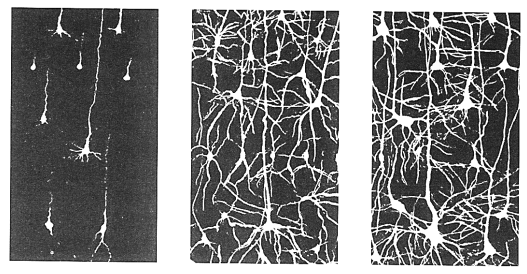
\includegraphics[scale=0.8]{sections/machine-learning/images/neuronale-netze.png}
      \caption{Vernetzungen nach der Geburt, nach 3 Monaten und nach 15 Monaten}
\end{figure}
%https://www.uni-wuerzburg.de/fileadmin/06000060/04_Fort-_und_Weiterbildungen_Lehrkraefte/Herbsttagungen/Herbsttagung_2016/20161006_WS_04_Neurobiologie.pdf

Neue Informationen verbinden bereits bestehende Neuronen und altes Wissen wird erneuert. Außerdem wird mit oftmaligem Wiederholen das Netzwerk dichter, und man kann das Erlernte leichter abrufen, zugleich werden die neuen Informationen mit dem bereits existierenden Vorwissen besser kombiniert. \cite{LANP}

\subsubsection{Supervised Learning}

An einen Algorithmus werden gruppierte Daten übergeben, die neben einer Gruppe noch mehrere Merkmale beinhalten, um danach neue Datensätze zu klassifizieren oder zu regredieren. Die Bezeichnung ''Supervised'' (im Deutschen ''Überwachtes'') kommt daher, dass die Gruppen bereits vordefiniert sind und das Programm nicht selber welche erstellen muss. \cite{SL:online}

\begin{table}[H]
      \centering
      \resizebox{.7\textwidth}{!}{
            \begin{tabular}{|l|l|l|l|}
                  \hline
                  \textbf{Farbe} & \textbf{Form} & \textbf{Geschmack} & \textbf{Frucht} \\ \hline
                  rot            & herzförmig    & süß                & Erdbeere        \\ \hline
                  gelb           & oval          & säuerlich          & Zitrone         \\ \hline
                  rot            & rund          & süß                & Apfel           \\ \hline
                  grün           & rund          & säuerlich          & Apfel           \\ \hline
            \end{tabular}}
      \caption{Beispiel für gruppierte Daten als Tabelle; Merkmale: Farbe, Form, Geschmack; Gruppe: Frucht}
      \label{tbl:fruit-data}
\end{table}

Diese Art von Lernen kann man in zwei Typen aufteilen:

\begin{itemize}
      \item Klassifizierung
      \item Regression
\end{itemize}

\paragraph{Klassifizierungs} Probleme verwenden Algorithmen, um Daten einer bestimmten Kategorie zuzuteilen. Oft gibt es nur zwei Kategorien wie zum Beispiel Hund/Katze oder Ja/Nein, jedoch gibt es auch Fälle, wo eine Vorhersage mit einer Wahrscheinlichkeit zwischen 0 und 1 getroffen wird. Weiteres gibt es auch Situationen, wo zwischen einer großen Menge an Kategorien ausgewählt wird, zum Beispiel bei der Erkennung von handschriftlichen Ziffern, in diesem Beispiel würde es zehn Möglichkeiten geben.

\begin{figure}[H]
      \centering
      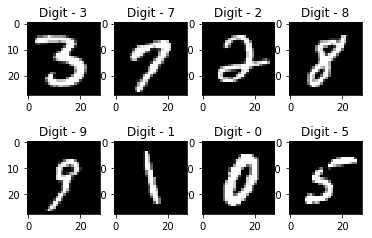
\includegraphics{sections/machine-learning/images/0_8-vKSQnZvKbtKXKy.png}
      \caption{Beispiel für eine Klassifizierung von handschriftlichen Ziffern}
      \label{ziffern}
\end{figure}
% https://aleenamishra10.medium.com/handwritten-digit-recognition-using-machine-learning-f6a08761ff83

Zu diesen ''überwachten'' Algorithmen gehören Lineare Diskriminanzanalysen, Support Vector Machines (SVM), Random Forests und Entscheidungsbäume.\cite{SL:online}

\subparagraph{Entscheidungsbäume} (Decision Trees) sind eine hierarchische Abfolge von Bedingungen und sind vergleichbar mit verschachtelten if/else-Statements. Dabei beginnt der Entscheidungsbaum mit einer Bedingung, die auch als ''Root-Node'' bezeichnet wird, worauf im Normalfall weitere Bedingungen folgen. Die Blätter dieser Pfade spiegeln die Gruppen oder Klassifizierungen wieder und sind nur über mehrere Pfade erreichbar.

Jedoch haben Entscheidungsbäume das Problem, dass sie sehr gut mit den antrainierten Daten arbeiten und weniger genau mit neuen Daten (Overfitting \ref{overfitting}). Um diese Genauigkeit zu verbessern, kann man zum Beispiel über Hyperparameter die maximale Länge eines Pfades setzen, wodurch die Bedingungen verallgemeinert werden.

\begin{figure}[H]
      \centering
      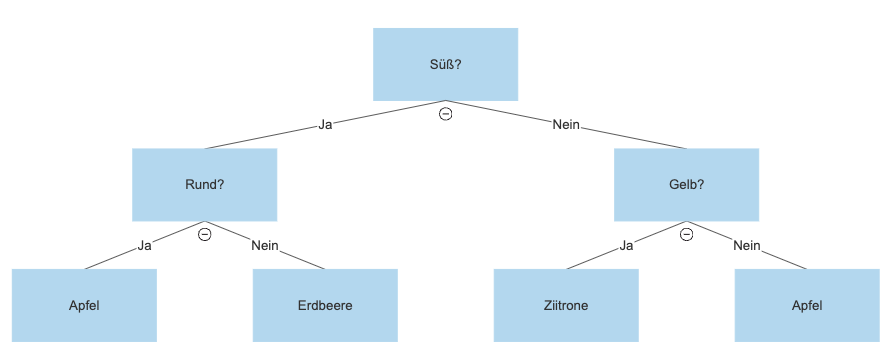
\includegraphics[scale=0.5]{sections/machine-learning/images/decision-tree.png}
      \caption{Decision Tree an dem Beispiel von Tabelle \ref{tbl:fruit-data}}
\end{figure}

In diesem Beispiel sieht dieser Entscheidungsbaum noch sehr lesbar aus, jedoch ändert sich dies, wenn Entscheidungen dargestellt werden, bei denen es auf die Nachkommastelle ankommt und wenn die Kategorien sehr schwer differenzierbar sind. Bei dem Supervised Learning erstellt das Programm selbstständig einen Entscheidungsbaum, indem es Muster oder Zusammenhänge findet und analysiert. Nach vielem Lernen kann dieser Entscheidungsbaum optimiert werden und unnötige Verbindungen können entfernt werden.

Fasst man mehrere Entscheidungsbäume zusammen, entsteht ein Random Forest, wobei jeder Entscheidungsbaum nur bestimmte Spalten/Merkmale zugeteilt bekommt. Soll ein neuer Datensatz kategorisiert werden, entscheidet die Mehrheit jener Ergebnisse der Entscheidungsbäume, zu welcher Gruppe dieser Datensatz dazugehört.

\paragraph{Regressionen,} Erstellung einer kontinuierlichen Funktion mithilfe von Werten, die auf oder nahe an der Funktion liegen, sind hilfreich, wenn anstatt diskreten kontinuierlichen Werte, wie zum Beispiel die Größe einer Person, festgestellt werden sollen. Dazu gehören lineare Regressionen und polynominale Regression.

\subsubsection{Unsupervised Learning}

Beim Unsupervised Learning oder unüberwachtes Lernen werden Verbindungen ohne genauere Informationen über den Testdatensatz erzeugt. Dabei muss das Programm selbst Gruppen definieren und dann die übergebenen Daten in diese Gruppen zuordnen. \cite{SL:online}

\paragraph{Clustering} gehört zu den beliebtesten Varianten, um selbstständig Gruppen zu erstellen. Dabei wird jeder Datensatz als Punkt in ein Koordinatensystem mit beliebig vielen Dimensionen eingetragen. Eine Achse stellt ein Attribut dar und je nach Ausprägung ist der Punkt mehr oder weniger vom Ursprung entfernt.

\begin{figure}[H]
      \centering
      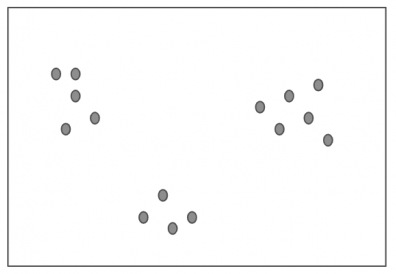
\includegraphics[scale=0.8]{sections/machine-learning/images/unclustered-data.png}
      \caption{Unkategorisierte Daten}
      \label{fig:unclustered-data}
\end{figure}
%https://datascience.eu/de/maschinelles-lernen/clustering-algorithmen-und-ihre-bedeutung-beim-maschinellen-lernen-2/

Auch für das menschliche Auge ist es möglich, dieses Beispiel (Abbildung \ref{fig:unclustered-data}) in Haufen oder Klumpen zusammenzufassen, genau das gleiche macht ein Programm mit Clustern. Die Interpretation dieser Gruppen muss jedoch wieder durch Menschen erfolgen, da ein Computer nicht im Stande dazu ist, diese Cluster einer Kategorie zuzuteilen.

Diese Vorgehensweise wird oft in sehr komplizierte Einsatzbereiche genutzt und daher ist es sehr schwer, differenzierbare Cluster zu erstellen. Der Prozess, solche Cluster zu definieren, basiert darauf, die Punkte so zu gruppieren, dass der Abstand in diesem Cluster klein ist und zu anderen Clustern groß.

\begin{figure}[H]
      \centering
      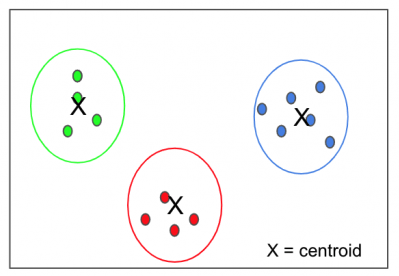
\includegraphics[scale=0.8]{sections/machine-learning/images/clustered-data.png}
      \caption{Kategorisierte Daten}
      \label{fig:clustered-data}
\end{figure}

\subsubsection{Reinforcement Learning}

Das Reinforcement Learning oder das beschränkte/verstärkte Lernen wird oft mit dem Konzept ''Learning by doing'' verglichen, da es sich weniger auf das Ergebnis fokussiert und mehr auf Aktionen oder Vorgängen. Ein Beispiel für diese Vorgehensweise aus der Sicht eines Schülers ist das Üben vor einer Matheschularbeit. Wird während dem Üben ein Fehler gemacht, merkt man sich das Problem und passt sein Verhalten / seinen Rechenweg so an, dass dieser Fehler nicht mehr vorkommt. Diesen Vorgang nennt man auch negative Verstärkung. \cite{SL:online}

Dahingegen führen richtige Ergebnisse oder erwartete Reaktionen zu positiven Verstärkungen und man versucht dieses Verhalten zu wiederholen.

Durch negative und positive Verstärkungen wird das Verhalten verbessert, um den besten Weg zum Ziel zu finden. Bei komplexen Systemen kann dies selbstständig vom Programm gemacht werden, jedoch bei simpleren kann es geschehen, dass ein unnötig komplizierter Weg gefunden wird. In diesen Fällen schaut ein Supervisor dem Programm ''über die Schulter''.

\subsection{Probleme}

\subsubsection{Overfitting} \label{overfitting} bedeutet, dass ein Modell zu sehr an die Trainingsdaten angepasst ist und auf neue Daten falsche Ergebnisse liefert. Dies hat den Grund, dass das Modell zu lange mit dem Trainingsdatensatz gearbeitet hat und zu spezifisch wurde. Daher versucht man mit einer Verallgemeinerung über die Hyperparameter das Modell zu vereinfachen.

\subsubsection{Underfitting} bedeutet, dass ein Modell viel zu allgemein ist und nicht an die Trainingsdaten angepasst ist. Einerseits könnte es sein, dass das Modell nur kurz mit den Trainingsdaten gearbeitet hat, andererseits kann es sein, dass die Klassifizierung innerhalb des Trainingsdatensatzes eine starke Mehrheit zeigt. \cite{OFUF}

\subsection{Phasen}

Das Erstellen von einem \Gls{ml}-Modell wir in vier Phasen unterteilt, wo jede Phase eine bestimmte Aufgabe erfüllt.

\begin{enumerate}
    \item Vorbereitung der Daten / Preprocessing

          Jeder Anfang sollte mit einer Analyse der Daten anfangen. Dabei sollte man die Datentypen, die Anzahl der Daten oder Klassifizierungen und die Anzahl der fehlenden Werte zusammenzufassen und überblicklich darstellen (Tabellen oder Diagramme). Dies hat zwei wesentliche Gründe und einer davon ist, dass man sich mit den Daten vertraut macht und danach über ein gewisses Verstehen verfügt. Der zweite Grund ist, dass man im Verlauf der Phase die Daten so verarbeiten kann, dass man am Ende das beste Ergebnis erreicht.

          Diese Vorbereitung sollte mit stichprobenartige Daten angeführt und später durch verschiedene Strategien weitergeführt werden, die dazu dienen, entweder fehlende Daten zu bereinigen oder Ausreißer zu beseitigen.

          Wie man mit fehlenden Daten umgeht, kommt auf die Situation an.
          Hat man Zugang zu einer große Mengen an Daten könnte es sinnvoll sein, diese Daten zu löschen. Dabei bleibt die Frage offen, ob man die ganze Spalte (wenn alle fehlenden Werte in einer Spalte sind) löscht oder nur die betroffenen Zeilen. Falls die Entscheidung getroffen wird, dass die Spalte entfernt wird, muss man sich vergewissern, dass damit potenziell wichtige Daten verloren gehen. Ist die Anzahl der Datensätze jedoch klein, hat ma die Möglichkeit fehlende Werte mit dem Mittelwert oder Ähnlichem zu ersetzten, dieser kann aus allen Daten gebildet werden oder aus den Daten, die über die selbe Klassifizierung verfügen. Sind diese Mittelwerte nicht repräsentativ, kann dieser durch einen fixen Wert ersetzt werden. Ein Beispiel dafür wäre die Analyse eines Schlaganfall-Datensatzes, in Fällen eines Kindes ist zu vermuten, dass es nicht raucht und daher ist es vertretbar, dass man dafür den Wert 0/false einsetzt. Die letzte Möglichkeit ist, dass man diese Werte mithilfe eines \gls{ml}-Modells (Regression) bestimmt. \cite{MLkg}

          Das Gegenteil der fehlenden Werte sind doppelte Werte, diese können zur Überrepräsentierung von bestimmten Klassifizierung führen und sollten daher bereinigt werden. Bei ähnlichen Werte ist dies jedoch eine Interpretationssache, da es in manchen Situationen ein unbedachter Messfehler sein könnten. Ein Vorteil dieses Schrittes ist, dass man am Ende von jeder Klasse gleich viele Datensätze hat.

          Als nächstes wäre eine Analyse jeder einzelnen Spalte sinnvoll, anfangend mit dem Datentypen. Falls es sich um Enumerationswerte handelt, müssten diese in numerische Werte umgewandelt werden, außer es handelt sich um die Klassifizierungsspalte. Handelt es sich um eine Spalte, wessen Werte eine Rangfolge  (z.B.: gut, mittel, schlecht) darstellen, kann man diese mit einer Nummer zwischen 0 und 1 austauschen. Dabei ist zu beachten, dass der minimalste und maximalste Rang entweder den Wert 0 oder 1 zugeteilt bekommen und jeder Rang dazwischen einen Wert dazwischen. Sind es jedoch unabhängige Enumerationswerte könnte man mithilfe der One-Hot-Encoding Methode die Daten umwandeln, wo jeder Enumerationswerte eine extra Spalte bekommt und entweder mit 0/1 (false/true) befüllt ist. Außerdem sollten unterschiedlichen Einheiten angeglichen werden und jene textuelle Einheit aus dem Wert entfernt werden.

          Das letzte Problem sind Ausreißer, um diese zu identifizieren, müsste man die eigentlich Verteilung der Daten kennen. Danach vergleicht man verdächtigte Werte (meistens der größte oder kleinste Wert) zum Durchschnitt und entscheidet, ob es sich wirklich um unerklärliche Werte handelt. Diese können mit den gleichen Funktionen, wie bei fehlenden Werten, ersetzt werden.

    \item Visualisierung der Daten

          Die tabellarische Darstellung von Daten erschweren es dem menschlichen Auge Muster zu erkennen, um dies zu umgehen ist jede Art der Visualisierung hilfreich. Damit kann man schnell Insights und Gruppen identifizieren, außerdem kann sie auch bereits bei der Vorbereitung der Daten helfen, da man zum Beispiel mithilfe eines Boxplots Ausreißer deutlich schneller erkennen kann.

          Um dies noch leichter zu machen, ist es wichtig, dass die Farbpalette an die gegebene Situation angepasst ist, da es bei schlechter Repräsentation leicht zu Verwirrung kommen kann. Wie zum Beispiel beim Darstellen vom Wetter hier bietet sich die Farbe blau für Regen an und rot/gelb für Sonnenschein.

          Jedes Diagramm hat seine Vorteile und Nachteile, wie zum Beispiel beim Violinplot die Verteilung der Daten relativ zur Anzahl der gleichen Klassifizierung sehr gut dargestellt werden. Jedoch hat es den Nachteil, dass diese Darstellung oft irreführend sind, da sie relativ anstatt absolut ist.

          Um Zusammenhänge besser zu erkennen, kann man zwei Variablen in einem Diagramm darstellen.

    \item Training des Modells

          Der erste Schritt beim Trainieren ist die Einteilung von Trainingsdaten und Testdaten, hierzu wird eine Einteilung von 70\% zum Trainieren und 30\% zum Testen angestrebt.

          Es ist wichtig, dass die Testdaten eine ausgeglichene Anzahl von Daten pro Klassifizierung enthaltet, da es sonst zu einem unbalancierten Modell kommen könnte. Wie in \ref{overfitting} beschrieben wurde, kann sich ein Modell zu sehr an die übergeben Trainingsdaten anpassen, so, dass später die Testdaten nicht korrekt klassifiziert werden. Um dies vorzubeugen könnte man einen Teil der Testdaten als Validierungsdaten nutzen, welche die Anpassung der Hyperparameter möglich machen \cite{DatenZumTrainieren}.

          Es ist wichtig die Testdaten nur zum Testen zu benutzten, da ab dem Moment, wo das Modell diese Daten verarbeitet schon gespeichert hat und im späteren Verlauf ebenfalls zur Klassifizierung nutzt.

          Am Anfang sollte man sich für einen traditionellen Algorithmus entscheiden, damit man später jegliche Veränderungen mit einem Basiswert vergleichen kann.

    \item Evaluierung und Verbesserung

          Um herauszufinden, ob das antrainierte Modell wirklich nutzvoll und genau ist, können folgende Werte berechnet und verglichen werden: Accuracy (Genauigkeit), Precision (Präzision) oder Recall. Je nach Situation sollte man den Fokus auf einen bestimmten Werte legen. Zum Beispiel beim Testen von Wasserqualitäten würde der wichtigste Wert die Precision sein, denn man kann in Kauf nehmen, dass nicht schädliches Wasser als schädlich gekennzeichnet wird, die entgegengesetzte Situation wäre nicht akzeptabel. \cite{APR}

          \begin{figure}[H]
              \[ accuracy = \frac{correct\ predictions}{all\ predictions}  \]

              \[ precision = \frac{true\ positives}{true\ positives + false\ positives}  \]

              \[ recall = \frac{true\ positives}{true\ positives + false\ negatives}  \]

              \caption{Formeln für Accuracy, Precision und Recall}
          \end{figure}

          Nachdem das Modell mit den Testdaten überprüft wurde, kann man beurteilen, ob die Genauigkeit die Erwartungen erfüllt. Falls dies nicht der Fall ist, bestehen 3 Möglichkeiten die Genauigkeit zu verbessern.

          Als erstes kann man die ausgewählte Vorgehensweise für fehlende oder ausreißende Daten ändern oder anpassen und die zweite Möglichkeit ist es den Algorithmus des Modells zu ändern. Am Ende kann man noch selbständig die Hyperparameter anpassen, was jedoch ein mühseliger Prozess sein kann, um ihn zu verkürzen kann man einen dieser Ansätze verwenden: Gridsuche, Zufallssuche, Bayessche Optimierung, Gradientenbasierte Optimierung oder Evolutionäre Optimierung. \cite{MLkg}
\end{enumerate}

\subsection{Optical Character Recognition}

In den meisten Fällen erfolgt eine Eingabe über eine Tastatur, jedoch ist dies manchmal weder die beste noch effizienteste Art, Text einzulesen. Mithilfe von \gls{ocr} ist ein automatisiertes Einlesen und Verarbeiten von handschriftlichen oder gedruckten Text möglich und das schon bereits in den 1950er. Am Anfang noch um Verkaufsberichte in Lochkarten zu konvertieren, damit ein Computer mit den Verkaufsdaten arbeiten kann \cite{OCR:online}.

Im Bereich von \gls{ocr} sind bereits momentan gute und präzise Resultate mit \glsfirst{ml} erwartbar, jedoch wie bei allen anderen Problem ist es verbesserbar. Um einen großen Fortschritt zu erreichen, würde die Nutzung von Deep Learning verpflichtend sein, dies ist jedoch in den meisten Situationen nicht notwendig.

Die Präzision hängt von vielen Attributen ab, daher kann ein eingescannter Text viel besser verarbeitet werden, als ein in der Freien geschossenes Bild mit dem Fokus auf ein Straßenzeichen \cite{OCR2:online}. 

\begin{itemize}
    \item Textdichte 
    
    Es macht einen Unterschied wie viel Text sich auf einer Fläche oder einem Bild befindet, denn es ist in gewissen Situationen leichter Text auszulesen, wenn dieser nur spärlich vorkommt. 
    \item Struktur
    
    Wenn man eine klare Struktur erkennt, zum Beispiel in Tabellen oder in Zeilen, kann man ein besseres Ergebnis erwarten, daher ist es auch wichtig, dass man vor dem Auslese-Prozess das übergebene Bild aufbereitet und als Beispiel die Rotation ändert. 
    \item Schriftart
    
    Handgeschriebene Texte oder ''laute'' Schriftarten sind im Gegensatz zu einfachen und gedruckten viel komplizierter, da sie kaum strukturiert sind. Außerdem könnten Buchstaben Ähnlichkeiten aufweisen, was später zu Verwechslungen führen kann.
    \item Buchstaben
    
    Sprachen wie Arabisch, Chinesisch, Russisch oder Japanisch benutzen im Gegensatz zu Deutsch ein anderes Alphabet, dabei kann es zu ähnlichen Buchstaben und Vertauschungen kommen, daher sinkt die Präzision in Texten mit mehreren Sprachen. Dies kann auch der Fall sein, wenn mathematische Formeln vorkommen.

    \begin{table}[H]
        \centering
        \begin{tabular}{|l|l|}
            \hline
            Kyrillisches Alphabet & Ähnelt dem Buchstaben im lateinischem Alphabet  \\ \hline
            \foreignlanguage{russian}{r} & p \\ \hline
            \foreignlanguage{russian}{V} & B \\ \hline
            \foreignlanguage{russian}{N} & H \\ \hline
            \foreignlanguage{russian}{U} & y \\ \hline
            \foreignlanguage{russian}{S} & C \\ \hline
        \end{tabular}
        \caption{Ähnlichkeiten zwischen Buchstaben im Lateinischem und Kyrillischem Alphabet}
    \end{table}
    \item Platzierung
    
    Zentrierte Texte erlauben ein besseres Auslesen, als abgeschnittene oder verstreute Wörter.
\end{itemize}

Die Texterkennung ist generell in zwei Phasen aufgeteilt:

\begin{itemize}
    \item Text Detection
    \item Text Recognition
\end{itemize}

\subsubsection{Text detection} ist der Prozess, indem in einem Bild oder einer PDF erkannt wird, wo sich Text befindet. Beim Resultat handelt es sich um Bounding Boxen, diese schließen einen Textblock (Wort, Buchstabe oder Paragraph) ein, dabei werden die genauen Koordinaten der Eckpunkte zurückgegeben. Diese werden später genutzt, um zur Visualisierung Boxen auf dem Bild oder der PDF aufzuzeichnen. Dieser Prozess wird auch in der Objekterkennung genutzt.

\begin{figure}[H]
    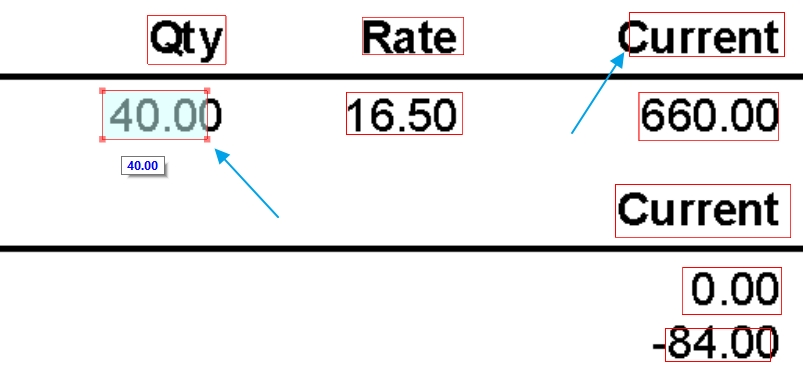
\includegraphics[scale=0.5]{sections/machine-learning/images/bounding-boxes.png}
    \caption{Bounding Boxes Beispiel}
    \label{fig:bounding-boxes}
\end{figure}

Die Erkennung kann entweder mittels der auf Regionen basierenden oder Textur basierenden Methode durchgeführt werden.

Bei der Regionen basierten Methode, werden Pixel verbunden und als Zeichenkandidat markiert, welche später mehrmals gruppiert werden und schlussendlich Wörter oder Textzeilen bilden. Dabei kommt es auf die geometrischen Eigenschaften an, wo es zu Fehlern beim Gruppieren kommen könnte. Wie man bei Abbildung \ref{fig:bounding-boxes} sehen kann, wurde der Buchstabe ''C'' im Wort ''Custom'' oder die letzte Nachkommastelle bei ''40.00'' nicht ganz als Teil des Wortes oder der Zahl erkannt.

Mit dem \Gls{swt} wird jedem Pixel eine Strichbreite zugeteilt, indem zwei Kanten gefunden werden mit der gleichen Richtung modulo 180°. Die Entfernung dieser zwei Kanten werden in den Kantenpixeln und alle unterliegenden Pixeln als Strichbreite gespeichert und alle Zusammenliegeden, gleich breite Pixel werden zu einem Zeichenkandidaten gruppiert. Danach werden alle benachbarten Zeichenkandidaten untersucht und zu einem Wort gruppiert, falls das mittelwertige Strichbreite-Verhältnis nicht über 2 liegt. Außerdem wird die Höhe und Farbe des Zeichenkandidaten berücksichtigt. Dies kann auch der Grund sein, wieso bei Abbildung \ref{fig:bounding-boxes} das Minuszeichen bei ''-84.00'' nicht zur Zahl hinzugefügt wird, das Minuszeichen ist signifikant niedriger als der Rest der Zahl. \cite{SWT:online}

\begin{figure}[H]
    \centering
    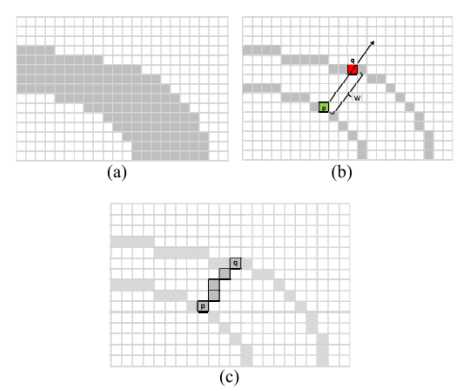
\includegraphics[scale=0.7]{sections/machine-learning/images/SWT.png}
    \caption{Die Kanten des Striches (a) werden solange verglichen, bis zwei gefunden werden mit der mit der gleichen Richtung (b). Alle unterliegenden Pixel erhalten die Strichbreite der Entfernung zwischen der Start- und Endkante (c).}
\end{figure}

Textur basierte Methoden unterteilen das Bild in Fester, dessen Höhe wird später mit der geschätzten Textgröße verglichen. Dabei kann es ebenfalls zu Erkennungsfehlern kommen.

Die Mischung dieser beiden Methoden gewann im Jahr 2011 den ICDAR-Wettbewerb \ref*{ICDAR} mit einem F-Score von 71.28\%. Hierbei hat Chunghoon Kim den Vorschlag gegeben, dass als erstes Blöcke  mit dem \Gls{mser} Verfahren extrahiert und danach benachbarte Blöcke gruppiert werden, falls die Farbe und Größe sich ähnelt. Jedoch werden mit diesem Verfahren, ebenfalls eine große Menge an false-postive Blöcken erkannt. Um diese Anzahl zu verringern wird eine ähnlich Idee zur \gls{swt} verwendet. \cite{SWT:online}

\paragraph{Wettbewerbe}\label{ICDAR} sind ein großer Grund für die Fortschritte in der Texterkennung und im Rahmen des zwei-jährlich stattfindenden \Gls{icdar} Wettbewerbs wurden alle oben genannten Ideen verglichen \cite{ICDAR:online}.

\subsubsection{Text Recognition} ist genau wie bei der Erkennung von Text in zwei Möglichkeiten unterteilt: Regionen basierend und Textur basierend. 

Die von \gls{mser} generierten und normalisierten Blöcke werden je nach der Orientierung in ein seerates Bild extrahiert. Dabei sind acht Orientierung möglich, welche mit ein Gaußschem Filter bearbeitet werden und auf ein 5 x 5 Bild komprimiert wurden. Mit diesen 5 x 5 x 8 = 200 dimensionalen Vektoren werden, dann die bereits erkannten Blöcke klassifiziert. \cite{SWT:online}


\subsection{Natural Language Processing}

\gls{nlp} gehört zu den Disziplinen der künstlichen Intelligenz, welche konstant...
